% HEREHEREHERE
% Author: Izaak Neutelings (May 2020)
% Inspiration: https://tex.stackexchange.com/questions/285578/how-to-draw-parallelepiped-and-cube-with-latex/288101#288101
% \documentclass[border=3pt,tikz]{standalone}
%%% HEREHEREHERE

\documentclass{article}
\usepackage{tikz}
\usepackage{fancyhdr}              %% headers/footers
\usepackage{makeidx}             %% Make an index uncomment following line
\usepackage[bookmarks]{hyperref} %% Make huperlinks within a PDF
\usepackage{color}                %% colored letters {\color{red}{{text}}
\usepackage{fancyhdr}              %% headers/footers
\usepackage{fancybox}              %% headers/footers


%%%%%%%%%%%%%%%%%%%%%%%%%%%%%% Setup Page %%%%%%%%%%%%%%%%%%%%%%%%%%%%%%%%%%%
%% \usepackage[paperheight=7.31in,paperwidth=9.5in,
%%   footskip=.05in,margin=.75in,
%%   includehead,includefoot,heightrounded
%% ]{geometry}

\usepackage[footskip=.05in,margin=.75in,
  includehead,includefoot,heightrounded
]{geometry}

\def\drafttest{DRAFT}
\def\wgdocdate{06 Oct, 2018}
\def\wgdocdatetime{\wgdocdate at \currenttime}
\ifx\documentisdraft\drafttest
\usepackage[left]{lineno}   %%%%%%%%%%%%% DRAFT
\usepackage{draftwatermark}
%%\SetWatermarkScale{5.0}
%%\SetWatermarkColor[gray]{0.3}
\fi

\usepackage{makeidx}             %% Make an index uncomment following line
\usepackage[bookmarks]{hyperref} %% Make huperlinks within a PDF
\usepackage{glossaries}          %% make a glossary
\renewcommand{\glossarypreamble}{"Glossary of Terms"}
\makeglossaries
\def\footerfilename{Glossary.tex}

%%\section{Glossary}

\newglossaryentry{noise}{name={noise},description={From \dhl{scombine} help: ``Values that are mixed into the record of a signal that originates as part of the system. Various strategies, philosophies and techniques are used to extimate the value. The noise characteristics of the \\
spectra can be described by fixed gaussian noise, a poissonian noise\\
which scales with the square root of the intensity, and a sensitivity\\
noise which scales with the intensity.''\\
$\sigma = \sqrt{\left(\frac{<\tt{I}>}{\tt{GAIN}} \right ) + \left( \frac{\tt{RDNOISE}}{\tt{I}} \right )^{2}  + (\tt{SENNOISE}\; \times <\tt{I}>)^{2}}$\\
\\
using RDNOISE, GAIN, and ``sensitivity noise''. Note: RDNOISE and GAIN\\
and intensity (I) are in ADU (DN) and require scaling by GAIN.  The\\
``sensitivity noise'', taken from flats, is a ``fraction''.}}

\newglossaryentry{analysis}{name={analysis},description={Action performed on a fully reduced file.}}

\newglossaryentry{apall}{name={apall},description={A IRAF task used to define apertures, extract the trace, determine and subtract background information, and to describe the trace using various fitting math functions: spline, spline3, chebyshev, legendre.}}

\newglossaryentry{apertures}{name={apertures},description={Apertures are assigned to each individual star's trace or the order of an echelle spectrum.}}

\newglossaryentry{background}{name={background},description={Noise, light pollution, spectral lines from city lamp sources, etc. Subtracted from source information in an image and characterized by its own noise statistics.}}

\newglossaryentry{band}{name={band},description={In IRAF, a subsets of information related to the data. In multispec spectra, band 1) is the final signal; 2) the raw signal before corrections; 3) the sky area; and 4) the SNR for the data.}}

\newglossaryentry{beam}{name={beam},description={A record from a separate optical path/sensor combination that may appear in certain instrument's spectral images.}}

\newglossaryentry{calibration}{name={calibration},description={The act of assigning a \textbf{\emph{W}}orld \textbf{\emph{C}}oordinate \textbf{\emph{S}}ystem to data.}}

\newglossaryentry{combine}{name={combine},description={In IRAF the combination of data from two or more images.}}

\newglossaryentry{command}{name={command},description={Incomputing, an imperative subject to qualification by parameteres, to accept data from a source (stdin), and send results to an output (stdout). }}

\newglossaryentry{commands}{name={commands},description={One or more command imperatives. They may be collected together into a 'script' and replayed  to affect at a later time.}}

\newglossaryentry{database}{name={database},description={An organized collection of data and inter-relationships stored in a management framework. Popular databases include Maria DB, PostgreSQL, etc.}}

\newglossaryentry{default}{name={default},description={A value used for a parameter, when no overide is provided.}}

\newglossaryentry{FITS}{name={fits},description={\textbf{\emph{F}}lexible \textbf{\emph{I}}mage \textbf{\emph{T}}ransport \textbf{\emph{S}}ystem Several forms: SIMPLE, \textbf{\emph{M}}ultiple \textbf{\emph{E}}xtension \textbf{\emph{F}}ile (MEF), Cube.}}

\newglossaryentry{flat}{name={flat},description={A special image file used to capture the vignetting profile, dust, and other defects unrelated to a source as seen by a sensor.}}

\newglossaryentry{function}{name={function},description={A name for an algorithm and its encapsulating logic. Used together with general logic forms tasks and programs.}}

\newglossaryentry{GAIN}{name={gain},description={A FITS value used to correct a 16-bit image pixel's value to the electron-count (inferred photon count) from a source as recorded by the sensor.}}

\newglossaryentry{header}{name={header},description={One of two parts of a FITS image extent, carrying information in 80 character cards (extents. think computer punch card) grouped together into blocks of 36 cards. Each entry consists of a keyword, value, and comment. Special cards for HISTORY and COMMENT follow different rules. The HEADER stops with a card with the END as its keyword. Blank cards are filled with 0x20 characters (spaces) not 0x00 (NULL).}}

\newglossaryentry{hedit}{name={hedit},description={The IRAF used to modify, extend or delete cards from a FITS header.}}

\newglossaryentry{histogram}{name={histogram},description={A binning of data, where the ordinal value is a value and the abscissa (reversed sense from algebra). Used to denote frequency of occurance of a value in a dataset.}}

\newglossaryentry{IMAGETYP}{name={imagetyp},description={IRAF tasks use a set of definitions. These are BIAS, DARK, FLAT, DOMEFLAT, SKYFLAT, IMAGE, COMPARISON etc. There are built in meanings to some, and offered by sites to help direct action of their specific packages.}}

\newglossaryentry{IRAF}{name={iraf},description={The Image Reduction and Analysis Facility. A collection of packages, tasks and proceedures created to reduce data from a particular instrument. May be used in very specific or loose general ways.}}

\newglossaryentry{MEDIAN}{name={median},description={Used here mainly to describe the value value falling between the minimum and maximum value in a dataset as described by a statistical approach.}}

\newglossaryentry{MODE}{name={mode},description={Used here mainly to describe the most common value in a dataset as described by a statistical approach.}}

\newglossaryentry{NAXIS}{name={naxis},description={A FITS keyword, found in an image, that describes the dimensions of the data. Value: 1) like a spectrum; 2) like an image; and 3) a datacube.}}

\newglossaryentry{object}{name={object},description={The target of an observation.}}

\newglossaryentry{OBJNAME}{name={objname},description={FITS - a significant keyword denoting the catalog or list name for a target.}}

\newglossaryentry{observations}{name={observations},description={A set of data, usually taken during one section on one date, at one site, of one or multiple targets; together with calibration and other instrumentation data.}}

\newglossaryentry{package}{name={package},description={A collection of parameters, tasks, help files within IRAF.}}

\newglossaryentry{parameters}{name={parameters},description={The information in the form of switches on a command line, values in a parameter file, etc that inform and alter the way a task proceeds with its actions.}}

\newglossaryentry{pixels}{name={pixels},description={A single element of a sensor. }}

\newglossaryentry{profile}{name={profile},description={In IRAF, a list of aperture profile images, the shape of data like a Point Spread Function for a star, a gaussian fit 'profile' centered around a point of interest, the general shape of a descriptive curve. }}

\newglossaryentry{pyraf}{name={pyraf},description={The newest, latest and probably final version of cl -- the IRAF command language.}}

\newglossaryentry{pyraflogin}{name={pyraflogin},description={A user supplied file, containing data, functions and tasks for use with PyRAF.}}

\newglossaryentry{Python}{name={python},description={Python is not a programming language as it is more of a programming envionment. The environment is richly awarded functionality. Care should be exercised as 'programs' developed under one version may not easily port to another.}}

\newglossaryentry{regions}{name={regions},description={Subsections of a 1D or 2D images.}}

\newglossaryentry{rejection}{name={rejection},description={Pixels that are discarded (and should be noted/recorded) from reduction and analysis.}}

\newglossaryentry{science}{name={science},description={IRAF - a shorthand way to describe an image carrying the information about sources in the sky.}}

\newglossaryentry{scombine}{name={scombine},description={The IRAF task to combine spectra, in the same way 2d images are aligned by the combine task.}}

\newglossaryentry{sigma}{name={sigma},description={The square root of the variance, defined in different ways by different statistical approaches.}}

\newglossaryentry{spectrum}{name={spectrum},description={A reduced trace from a star, imaged by a spectrograph. May be instrumental (not corrected) or complete with wavelength and energy calibration.}}

\newglossaryentry{standard}{name={standard},description={A short-hand way to refer to a standard (pre measured and described) reference star.}}

\newglossaryentry{stdout}{name={stdout},description={Unix: the file stream where nominal messages are written, as to the terminal or redirected to a file.}}

\newglossaryentry{task}{name={task},description={A 'function' within a package within IRAF.}}

\newglossaryentry{target}{name={target},description={See OBJNAME.}}

\newglossaryentry{trace}{name={trace},description={The path of a star's image across a sensor in the same beam.}}

\newglossaryentry{Unix}{name={Unix},description={The operation system, a play on words from the Multics operating system. The OS of IRAF.}}

\newglossaryentry{WCS}{name={WCS},description={\textbf{\emph{W}}orld \textbf{\emph{C}}oordinate \textbf{\emph{S}}ystem: a function that maps a sensor's x,y and sometimes z axis into RA/Dec or Angstroms etc. The Z axis may contain time data by wavelength for example.}}


%%%%%%%%%%%%%%%%%%%%%%%%%%%%%%%%%%%%%%%%%%%%%%%%%%%%%%%%%%%%%%%%%%%%%%%%%%%%%
\hypersetup{
    colorlinks  = true,
    linkcolor   = blue,
    citecolor   = red,
    urlcolor    = blue,
    pdfauthor   = {Copyright(c) 2018-22. All rights reserved. Wayne Green},
    pdftitle    = {PyRAF/IRAF/Unix 2.17.1 PyRAF 3 “Bon Mots”},
    pdfsubject  = {Collection of Notes for IRAF},
    pdfkeywords = {Phoptometry, Spectrography,IRAF},
    pdfcreator  = {LaTeX with hyperref package},
    pdfproducer = {dvips + ps2pdf}
}

%%%%%%%%%%%%%%%%%%%%%%%%%%%%%%%%%%%%%%%%%%%%%%%%%%%%%%%%%%%%%%%%%%%%%%%%%%%%%

\usetikzlibrary{math}
\usetikzlibrary{arrows,arrows.meta}
\usetikzlibrary{calc,shapes, shapes.geometric}
\usetikzlibrary{intersections}
\usetikzlibrary{fadings}
\usetikzlibrary{decorations.markings}
\usetikzlibrary{angles,quotes} % for pic (angle labels)
\usetikzlibrary{backgrounds}

%\usepackage{tkz-euclide} % for \tkzMarkRightAngle
%\usetkzobj{all}

\colorlet{myblue}{blue!80!black}
\colorlet{mydarkblue}{blue!35!black}
\colorlet{myred}{black!50!red}
\colorlet{glasscol}{blue!10}
\colorlet{Ecol}{orange!90!black}
\tikzset{>=latex} % for LaTeX arrow head
\tikzstyle{ray} = [line width = 0.85, color = red]
\tikzstyle{vertical} = [line width = 0.85, dashed]
\tikzstyle{myarr}=[-{Latex[length=3,width=2]}]
\tikzstyle{Evec}=[Ecol,{Latex[length=2.8,width=2.5]}-{Latex[length=2.8,width=2.5]},line width=0.6]
\tikzstyle{glass}=[top color=glasscol!88!black,bottom color=glasscol,shading angle=0]
%\tikzstyle{glass}=[top color=glasscol!88!black,bottom color=glasscol,middle color=glasscol!98!black,shading angle=0]
\tikzset{
  light beam/.style={thick,myblue,decoration={markings,
                     mark=at position #1 with {\arrow{latex}}},
                     postaction={decorate}},
  light beam/.default=0.5}

\newcommand{\lline}[4]{\draw[vertical] (#1) -- ({#2*cos(#4)-#3*sin(#4)},{+#2*sin(#4)+#3*cos(#4)});}


\newcommand\rightAngle[4]{
  \pgfmathanglebetweenpoints{\pgfpointanchor{#2}{center}}{\pgfpointanchor{#3}{center}}
  \coordinate (tmpRA) at ($(#2)+(\pgfmathresult+45:#4)$);
  \draw[white,line width=0.6] ($(#2)!(tmpRA)!(#1)$) -- (tmpRA) -- ($(#2)!(tmpRA)!(#3)$);
  \draw[blue!40!black] ($(#2)!(tmpRA)!(#1)$) -- (tmpRA) -- ($(#2)!(tmpRA)!(#3)$);
}

%-----------------------------------------------------------------------------
% tikz/prisms2.tikz
%% Incident Ray
\tikzstyle{ray} = [%
					line width = 0.85, 
					color = red,
					postaction = decorate, decoration={markings, mark=at position .52 with \arrow{stealth}}
					]
%% Refracted Ray
\tikzstyle{ray1} = [%
					line width = 0.85, 
					color = red]
%% Dashed
\tikzstyle{vertical} = [%
					line width = 0.85, 
					dashed]

%-----------------------------------------------------------------------------
% Huygens.tikz -- WAVEFRONT
% store in -- defines a special TeX macro
\def\p{0.03}
\def\r{0.25}
\tikzset{
  wavefront/.pic={
     \tikzset{/wavefront/.cd,#1}
     \fill (0,0) circle (\p);
     \draw (\wang:\r) arc(\wang:-\wang:\r);
  }
  /wavefront/.search also={/tikz},
  /wavefront/.cd,
  ang/.store in=\wang, ang={60},
}

%%%%%%%%%%%%%%%%%%%%%%%%%%%%%%%%%%%%%%%%%%%%%%%%%%%%%%%%%%%%%%%%%%%%%%%%%%%%%
%%%%%%%%%%%%%%%%%%%%%%%%%%%%%%%%%%%%%%%%%%%%%%%%%%%%%%%%%%%%%%%%%%%%%%%%%%%%%
%%%%%%%%%%%%%%%%%%%%%%%%%%%%%%%%%%%%%%%%%%%%%%%%%%%%%%%%%%%%%%%%%%%%%%%%%%%%%

% Good source of pre-cooked tikz images.
% https://github.com/Expander/tikz-images/tree/master/optics
\pagestyle{fancy}
\fancyhf{}
\providecommand\footerfilename{}
\renewcommand\footerfilename{BonMots.tex}
\fancyfoot[LF,OLF]{Go to: \hyperref[sec:contents]{Contents}}
\fancyfoot[RF,ORF]{Go to: \hyperref[sec:index]{Index~\footerfilename}}
\fancyfoot[CF,OCF]{Page \thepage~~~ \footerfilename}


\begin{document}
\pagenumbering{gobble}   %ignore page numbers for a while
\setlength{\footskip}{13.59999pt}

\title{BonOptics}
\author{\vspace{-0.2cm} Wayne Green}
\date{\vspace{-0.2cm} \today}
\maketitle

\begin{abstract}
Notes on Optics related to spectroscopy and optics in general.
\end{abstract}

%%%%%%%%%%%%%%%%%%%%%%%%%%%%%%%%%%%%%%%%%%%%%%%%%%%%%%%%%%%%%%%%%%%%%%%%%%%%%
%% table of contents
%%%%%%%%%%%%%%%%%%%%%%%%%%%%%%%%%%%%%%%%%%%%%%%%%%%%%%%%%%%%%%%%%%%%%%%%%%%%%

\pagenumbering{roman}   % i,ii,etc
\pagenumbering{gobble}   %ignore page numbers for a while
\pdfbookmark[0]{Table of Contents}{MyTOC} % if usepackage{hyperref} in use.

\section*{~} \label{sec:contents}
\tableofcontents
\listoffigures
\listoftables

\clearpage
\pagenumbering{arabic}
\providecommand\footerfilename{}
\renewcommand\footerfilename{BonOptics.tex}
\fancyfoot[LF,OLF]{Go to: \hyperref[sec:contents]{Contents}}
\fancyfoot[RF,ORF]{Go to: \hyperref[sec:index]{Index~\footerfilename}}
\fancyfoot[CF,OCF]{Page \thepage~~~ \footerfilename}

\section{Overview}

In this document, angles will follow the standard sign convention of
positive angles with respect to (w.r.t.) their axis of rotation are considered
to be counter-clockwise and negative angles are clockwise (follows the rignt
hand rule).

$n_{x}$ represents the index of refraction of a medium. Vacuum is = 1.0. Other common
glass values appear in appendix \ref{sec:IndexRefractionTable}. Index of refraction
is a function of wavelength.

- maintain an injection f/ < NA of the fiber.


Fermat's  Principal Light  does  not take  the  shortest path  through
space, it  takes the fastest  path through time. Propagation  speed is
expressed with the index of refraction $n$.

\clearpage
\section{Snell's Law}

%  Borrowed from -- Refraction  Author: Jimi Oke
% /home/git/external/BonMots/tex/BonMots/tikz/snellslaw.tikz
\begin{figure}[h!]
\centering
\tikzstyle arrowstyle=[scale=1]
\tikzstyle directed=[postaction={decorate,decoration={markings,
    mark=at position .65 with {\arrow[arrowstyle]{stealth}}}}]
\tikzstyle reverse directed=[postaction={decorate,decoration={markings,
    mark=at position .65 with {\arrowreversed[arrowstyle]{stealth};}}}]

\begin{tikzpicture}

    % define coordinates
    \coordinate (O) at (0,0) ;
    \coordinate (A) at (0,4) ;
    \coordinate (B) at (0,-4) ;
    
    % media
    \fill[blue!25!,opacity=.3] (-4,0) rectangle (4,4);
    \fill[blue!60!,opacity=.3] (-4,0) rectangle (4,-4);
    \node[right] at (2,2) {Air};
    \node[left] at (-2,-2) {Water};

    % axis
    \draw[dash pattern=on5pt off3pt] (A) -- (B) ;

    % rays
    \draw[red,ultra thick,reverse directed] (O) -- (130:5.2);
    \draw[blue,directed,ultra thick] (O) -- (-70:4.24);

    % angles
    \draw (0,1) arc (90:130:1);
    \draw (0,-1.4) arc (270:290:1.4) ;
    \node[] at (280:1.8)  {$\theta_{2}$};
    \node[] at (110:1.4)  {$\theta_{1}$};
\end{tikzpicture}
\caption{Snell's Law}
\label{fig:SnellsLaw}

\end{figure}


% HEREHEREHERE

\clearpage
\include{BrewsterAngle.tex}

\clearpage
\section{Huygens' Principle}
% /home/git/external/BonMots/tex/BonMots/tikz/huygens.tikz
\begin{figure}[h!]
\centering
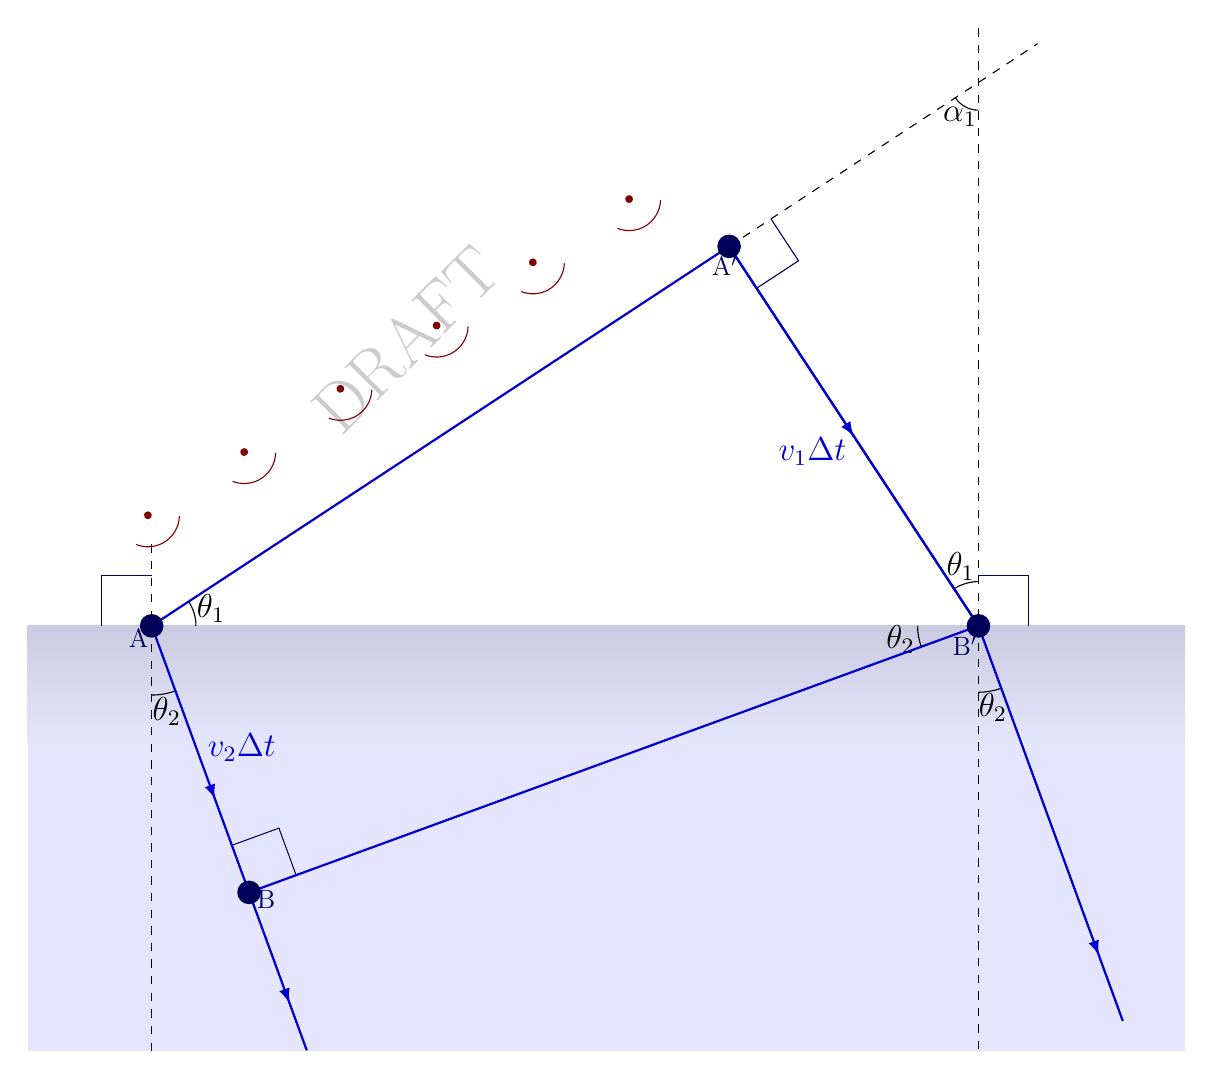
\begin{tikzpicture}[scale=3.0,font=\large]
  \def\N{6}                     % number of wavefronts
  \def\r{0.4}                   % wavefront radius
  \def\w{3.5}                   % width
  \def\h{2.3}                   % height
  \def\d{1.8}                   % depth
  \def\t{0.5}                   % thickness
  \def\l{1.78}                  % length light beam
  \def\p{0.05}                  % point size
  \def\ang{atan(\h/\w)}
  \def\ymin{-0.15*\w}
  \def\ymax{ 1.25*\w}
  \def\na{1.0}                  % index refraction air
  \def\ng{1.6}                  % index refraction glass
  \def\anga{20}
  \def\angg{asin(\na/\ng*\h/sqrt(\h^2+\w^2))}
  \def\sangg{\na/\ng*\h/sqrt(\h^2+\w^2)}
  \coordinate (O)   at (0,0);
  \coordinate (WR)  at (\w,0);
  \coordinate (WT)  at (\w,\h);
  \coordinate (L)   at (\ymin,0);
  \coordinate (R)   at (\ymax,0);
  \coordinate (T)   at (\w, 1.10*\h);
  \coordinate (B)   at (\w,-\d);
  \coordinate (BL)  at (0,-\d);
  \coordinate (TL)  at (0,0.15*\h);
  \coordinate (P)   at ($(WT)!(WR)!(O)$);
  \coordinate (F)   at ({\w+\l*cos(-90+\angg)},{\l*sin(-90+\angg)});
  \coordinate (VT)  at ({\w*\sangg*\sangg},{-\w*\sangg*cos(\angg)});
  %\coordinate (VI) at ({\w+\l*cos(180+\angg)},{\l*sin(180+\angg)});
  
  % MEDIUM
  \fill[glass] (L) rectangle (\ymax,-\t);
  \fill[glasscol] (\ymin,-0.99*\t) rectangle (\ymax,-\d);
  
  % ANGLE
  \rightAngle{WT}{WR}{R}{0.3}
  \rightAngle{WT}{P}{WR}{0.3}
  \rightAngle{O}{VT}{WR}{0.3}
  \rightAngle{L}{O}{TL}{0.3}
  \draw pic["$\theta_1$",draw=black,angle radius=16,angle eccentricity=1.4] {angle = R--O--WT};
  \draw pic["$\theta_1$",draw=black,angle radius=16,angle eccentricity=1.4] {angle = WT--WR--P};
  \draw pic["$\theta_2$",draw=black,angle radius=24,angle eccentricity=1.25] {angle = B--WR--F};
  \draw pic["$\alpha_1$",draw=black,angle radius=10,angle eccentricity=1.4] {angle = O--WT--WR};
  \draw pic["$\theta_2$",draw=black,angle radius=22,angle eccentricity=1.3] {angle = L--WR--VT};
  \draw pic["$\theta_2$",draw=black,angle radius=25,angle eccentricity=1.25] {angle = BL--O--VT};
  
  % LINES
  \draw[dashed] (TL) -- (BL);
  \draw[dashed] (T) -- (B);
  \draw[dashed] (P) -- (WT) --++ ({\ang}:0.3);
  \draw[light beam={0.65}] (O) -- (VT) node[midway,above=4,right=-1] {$v_2 \Delta t$};
  \draw[light beam={0.70}] (VT) --++ ({\angg-90}:0.4*\l);
  \draw[] (P) -- (WR) -- (F);
  \draw[light beam={0.50}] (P) -- (WR) node[midway,above=2,below left=-1] {$v_1 \Delta t$};
  \draw[light beam={0.92}] (P) -- (WR) -- (F);
  %\draw[] (WT) -- (WR);
  \draw[myblue,thick] (O) -- (P);
  \draw[myblue,thick] (VT) -- (WR);
  
  \fill[mydarkblue] (O) circle (\p) node[scale=0.8,below left=-2] {A};
  \fill[mydarkblue] (P) circle (\p) node[scale=0.8,left=2,below=1] {A$'$};
  \fill[mydarkblue] (VT) circle (\p) node[scale=0.8,below=3,right=0] {B};
  \fill[mydarkblue] (WR) circle (\p) node[scale=0.8,right=4,below left=1] {B$'$};
  
  % WAVE FRONTS
%  \foreach \i [evaluate={\x=-\r*sin(\ang)+\i*\w/(\N+1);
%                         \y=\r*cos(\ang)+\i*\h/(\N+1);}] in {1,...,\N}{
%    \pic[myred,rotate=\ang-90] at (\x,\y) {wavefront={ang={55}}};
%  }
  \foreach \i [evaluate={\f=(\i-0.5)/\N;}] in {1,...,\N}{
    \pic[myred,rotate=\ang-90] at ($(O)!\f!(P)+({\ang+90}:\r)$) {wavefront={ang={55}}};
  }
  
\end{tikzpicture}
\caption{Huygens Principle}
\label{fig:HuygensPrinciple}
\end{figure}



\clearpage
\include{ReflectionRefraction.tex}

\clearpage
\include{ReflectionRefractionBrewsterAngle.tex}

\clearpage
\section{Prisms}

% /home/git/external/BonMots/tex/BonMots/tikz/prism.tikz
% PRISM + REFRACTION
\begin{figure}[h!]
\centering
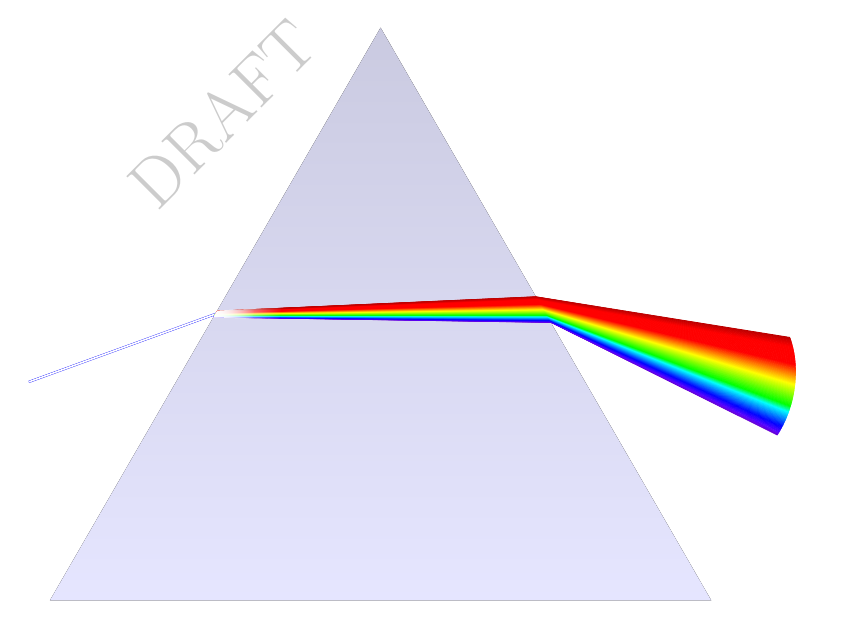
\begin{tikzpicture}[scale=3.0,font=\large]
  \def\N{200} % number of rainbow rays
  \def\L{2.8}
  \def\na{1.0} % air
  \def\angi{50}
  \coordinate (O) at (0,0);
  \coordinate (R) at (\L,0);
  \coordinate (T) at (60:\L);
  \coordinate (I) at (60:0.5*\L);
  
  % MEDIUM
  \draw[line width=0.8,blue]  (I)++(150+\angi:0.3*\L) -- (I) --++ (\angi-30:0.01*\L);
  \draw[line width=0.6,white] (I)++(150+\angi:0.3*\L) -- (I) --++ (\angi-30:0.01*\L);
  \fill[glass] (O) -- (T) -- (R) -- cycle;
  \path[name path=side] (T) -- (R);
  
  % LIGHT BEAMS
  % https://tex.stackexchange.com/questions/230227/creating-a-rainbow-color-macro
  \begin{scope}
    \coordinate (IT) at ($(I)+(60:0.006*\L)$);
    \clip (O) -- (T) -- (1.08*\L,0.45*\L) to[out=-35,in=20,looseness=1]
          (1.04*\L,0.2*\L) -- (R) -- cycle;
    \foreach \i [evaluate={
        \f=\i/\N;
        \ng=1.6-\f*0.2;
        \lamb=410+\f*320;
        \angr=asin(\na/\ng*sin(\angi));
        \angR=asin(\ng/\na*sin(60-\angr));
        \dl=0.0108*(1-\f)*\L;}] in {0,...,\N}{
      \definecolor{tmpcol}{wave}{\lamb}
      \colorlet{mycol}[rgb]{tmpcol}
      \path[name path=beam1] (I) --++ (-30.1+\angr:0.8*\L);
      \path[name path=beam2] (I) --++ (-30.0+\angr:0.8*\L);
      \coordinate (IT2) at ($(I)+(57:0.005*\L)+(-120:\dl)$);
      \fill[mycol,name intersections={of=side and beam1,name=t},
            name intersections={of=side and beam2,name=b}] %wave={\len}
        (IT2) -- (t-1) -- ($(t-1)+(30.0-\angR:0.4*\L)$)
        -- ($(b-1)+(30.1-\angR:0.4*\L)$) -- (b-1) -- ($(IT2)+(-120:-0.001*\L)$); %node[scale=0.3] {\angR};
    }
  \end{scope}
  \fill[white,path fading=east]
    (IT) --++ (-120:0.012*\L) --++ (-1.3:0.06*\L) --++ (80:0.015*\L) -- cycle;
  \fill[white,path fading=east]
    (IT) --++ (-120:0.012*\L) --++ (-1.3:0.10*\L) --++ (80:0.018*\L) -- cycle;
  
\end{tikzpicture}
\caption{Prism Refraction}
\label{fig:Prism}

\end{figure}


% /home/git/external/BonMots/tex/BonMots/tikz/prism90.tikz

\begin{figure}[h!]
\centering
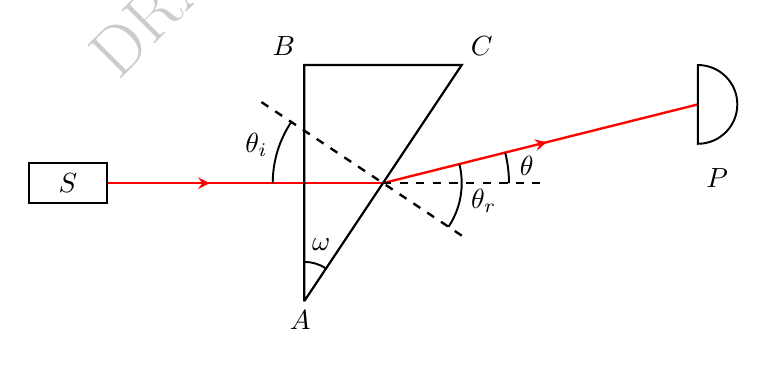
\begin{tikzpicture}[semic/.style args={#1,#2}{semicircle,minimum width=#1,draw,anchor=arc end,rotate=#2},outer sep=0pt,line width=.7pt]
	
	% Grid
    \iffalse
	\draw[dotted] (0,0) grid (10,10);
	\foreach \i in {0,...,10}
	{
		\node at (-2ex,\i) {\i};
		\node at (\i,-2ex) {\i};
	}
    \fi
	
	% Coordinates
	\coordinate (S)  at (1,1.5);
	\coordinate (P)  at (9,3);
	\coordinate (A)  at (4,1.5);
	\coordinate (B)  at (5,1.5);
	\coordinate (C)  at (6, 29/6-4);
	\coordinate (C') at (3.4, 2.56667);
	
	% Nodes
	%% Source
	\node[draw, rectangle, minimum width=1cm, minimum height=0.5cm] at (S) (s) {$S$};
	%% Detector
	\node [semic={1cm,-90}, label={[rotate=0, below left, yshift=-0.7cm]$P$}] at (P) {};
	
	% Prism
	\draw[thick] (4,0) coordinate (K) node [below, xshift=-0.05cm] {$A$} -- ++(0,3) coordinate (L) node [above left] {$B$}-- +(2,0) coordinate (M) node [above right] {$C$} -- (4,0);
	
	
	\begin{scope}[on background layer]
		% Rays
		\draw[ray] (s) -- (A);
		\draw[ray] (B) -- (9,2.5) coordinate (P');
		\draw[ray1] (A) -- (B);
		% Dashed
		\draw[vertical] (C) -- (C');
		\draw[vertical] (B) -- (7,1.5) coordinate (B');
	\end{scope}
	
	% Angles
	\pic[draw, "$\omega$", angle eccentricity=1.5] {angle={M--K--L}};
	\pic[draw, "$\theta_i$", angle eccentricity=1.2, angle radius=1.4cm] {angle={C'--B--S}};
	\pic[draw, "$\theta_r$", angle eccentricity=1.3, angle radius=1cm] {angle={C--B--P'}};
	\pic[draw, "$\theta$", angle eccentricity=1.15, angle radius=1.6cm] {angle={B'--B--P'}};
\end{tikzpicture}
\caption{Prism2.}
\label{fig:Prism2}
\end{figure}


\clearpage
\section{Young's Two Slitc Interference}

% /home/git/external/BonMots/tex/BonMots/tikz/interferrence.tikz

\begin{figure}[h!]
\centering
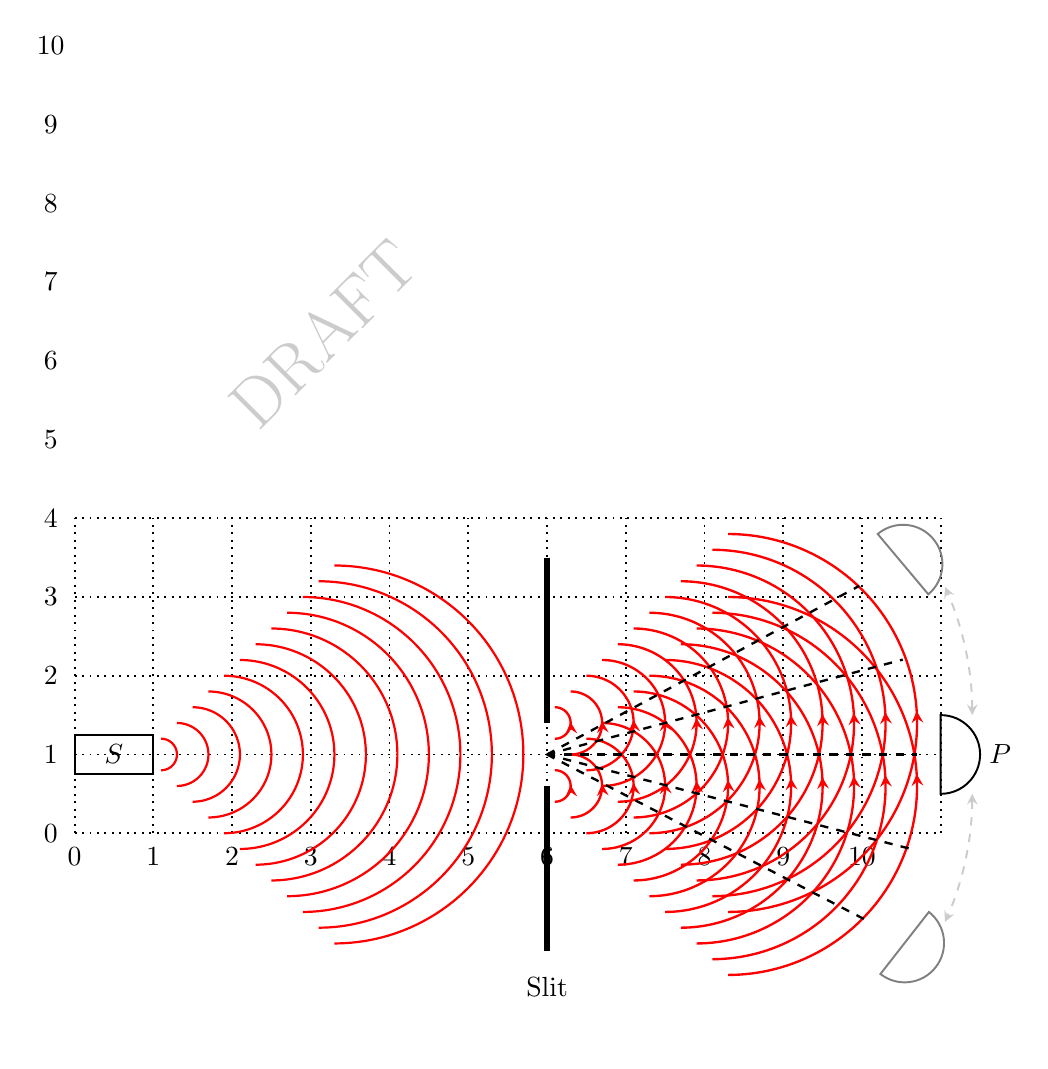
\begin{tikzpicture}[semic/.style args={#1,#2}{semicircle,minimum width=#1,draw,anchor=arc end,rotate=#2},outer sep=0pt,line width=.7pt]
	
	% Grid
	\draw[dotted] (0,0) grid (11,4);
	\foreach \i in {0,...,10}
	{
		\node at (-2ex,\i) {\i};
		\node at (\i,-2ex) {\i};
	}
	
	% Coordinates
	\coordinate (S) at (0.5,1);
	\coordinate (P) at (11,1.5);
	\coordinate (A) at (6,1);
	
	% Nodes
	\node[draw, rectangle, minimum width=1cm, minimum height=0.5cm] at (S) {$S$};
	\node (p')  [semic={1cm,-90}, label={[rotate=0, below left, yshift=-0.7cm, black!50]}, black!50, rotate=40] at (10.2,3.8) {};
	\node (p)   [semic={1cm,-90}, label={[rotate=0]$P$}] at (P) {};
	\node (p'') [semic={1cm,-90}, label={[rotate=0, below left, yshift=-0.7cm, black!50]}, black!50, rotate=-38] at (10.85,-1.) {};
	
	% Slit
	\draw[line width = 2] (6,3.5) -- (6,1.4);
	\draw[line width = 2] (6,-1.5) -- (6,0.6) node[below, pos=-0.1] {Slit};
	
	% Dashed Grey Lines
	\draw[stealth-stealth, black!20, dashed] (11.4,1.5) arc (0:24:4);
	\draw[stealth-stealth, black!20, dashed] (11.4,0.5) arc (0:-24:4);
	
	% Interference Pattern
	%% Before Slit
	\foreach \i in {0,0.2,...,2.2}
	{
		\draw [red,thick,domain=-90:90, samples=100] plot ({0.2*cos(\x)+\i*cos(\x)+1.1+\i}, {0.2*sin(\x)+\i*sin(\x)+1});
	};
	% After Slit
	\foreach \i in {0,0.2,...,2.2}
	{
		\draw [ray, domain=-90:90, samples=100] plot ({0.2*cos(\x)+\i*cos(\x)+6.1+\i}, {0.2*sin(\x)+\i*sin(\x)+1.4});
		\draw [ray, domain=-90:90, samples=100] plot ({0.2*cos(\x)+\i*cos(\x)+6.1+\i}, {0.2*sin(\x)+\i*sin(\x)+0.6});
	};
	
	% Black Dashed Lines
	\draw[vertical] (6,1) -- (10.7,1);
	\lline{6,1}{10.7}{1}{6.5};
	\lline{6,1}{10.4}{1}{12};
	\lline{6,1}{10.6}{1}{-6.5};
	\lline{6,1}{10.1}{1}{-12};

\end{tikzpicture}
	\caption{Young's two slit interference.}
\label{fig:Interferrence}

\end{figure}



\clearpage
\section{Echelle}

% /home/git/external/BonMots/tex/BonMots/tikz/echelle3.tikz
\begin{figure}[h!]
\centering
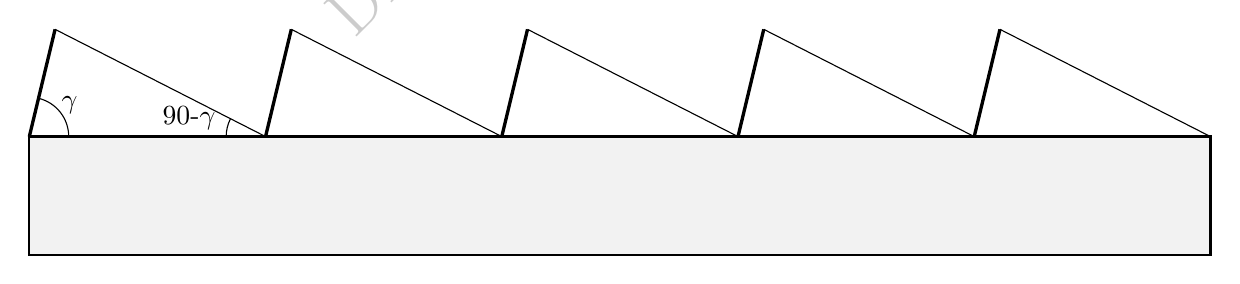
\begin{tikzpicture}[scale=3,>=Stealth]
    % Define style for incoming and diffracted raysa
    \tikzstyle{ray} = [thick,->]
    % /home/git/external/BonMots/tex/BonMots/tikz/echelle3.tikz
    
    % Grating parameters
    \def\lmm       {79}                % lines per mm of grating
    \def\blaze     {63}                % Blaze angle in degrees (e.g., 63 or 75 for echelle)
    \def\numsteps  {5}                 % number of rules to display
    \def\stepsize  {0.6}               % legacy
    \def\subheight {.5}                % height of substrate segment
    \def\subwidth  {5}                 % length of substrate segment
    \def\g         {1.0 / \lmm}        % computed 1 / lmm  % (iv (setq tmp (/ 1.0 79 )))    0.012658227848101266
    \pgfmathsetmacro{\bangle}{\blaze};   % *pi/180.0
    \pgfmathsetmacro{\xoffs}{1-cos(90.0-\blaze)};
    \pgfmathsetmacro{\yoffs}{\subheight+sin(90.0-\blaze)};

    \coordinate (origin) at (0,0);

    % Draw the echelle sawtooth profile (gross structure)
    \iffalse
        \draw[step=1cm, gray!50, very thin] (origin) grid (5,5);
        \fill (origin) circle (1pt);
        \foreach \x in {0,...,5} {
           \draw (\x,0) -- (\x,-0.1);
           \node[below] at (\x,-0.11) {$\x$};
        }

        \foreach \y in {0,...,5} {
           \draw (-.11, \y) -- (0,\y);
           \node[left] at (-0.11,\y) {$\y$};
        }
    \fi

    % Draw the bulk substrate block
    \draw[thick, fill=gray!10] (0,0) rectangle (5, .5);
    % draw the facets
    \draw[very thick] (0,\subheight) coordinate(A)-- (\xoffs, \yoffs)  coordinate(B); 
          \draw[thin] (\xoffs, \yoffs)   -- (1,\subheight) coordinate(C);
    \draw[very thick] (1,\subheight) -- (1+\xoffs, \yoffs); \draw[thin] (1+\xoffs, \yoffs) -- (2,\subheight);
    \draw[very thick] (2,\subheight) -- (2+\xoffs, \yoffs); \draw[thin] (2+\xoffs, \yoffs) -- (3,\subheight);
    \draw[very thick] (3,\subheight) -- (3+\xoffs, \yoffs); \draw[thin] (3+\xoffs, \yoffs) -- (4,\subheight);
    \draw[very thick] (4,\subheight) -- (4+\xoffs, \yoffs); \draw[thin] (4+\xoffs, \yoffs) -- (5,\subheight);
    \pic[draw, pic text={$\gamma$},angle eccentricity=1.3 ] {angle=C--A--B}; 
    \pic[draw, pic text={90-$\gamma$},angle eccentricity=2 ] {angle=B--C--A}; 








%%    \node[right] at (\xoffs+.2, \yoffs) {$gamma \bangle = (\xoffs,\yoffs)$};


%%       % Draw the sawtooth grating surface
%%       \draw[thick] (origin) 
%%       \foreach \i in {1,...,\numsteps} {
%%           -- ++(\stepsize, {-\stepsize*tan(\blaze-90)})   % steep face (shadow side) or adjust slope
%%           -- ++(-\stepsize*0.15, {\stepsize*tan(\blaze)}) % blaze face
%%       };


%%    \foreach \x [evaluate=\x as \y using {\x^2 - 1}] in {1,2,3} {
%%        \node at (\x, \y) {(\x, \y)};
%%    };

    
%%    % Draw the sawtooth grating surface
%%    \pgfmathsetmacro{\top}{\g*sin(\gamma)}
%%    \pgfmathsetmacro{\gcosgamma}{\g*cos(\gamma)}
%%    \draw[thick] (origin) 
%%    \foreach \x    [evaluate=\x as \y using {\g*cos(\gamma)}]  in {1,...,\numsteps} {
%%        -- ++(\x,\y)
%%        -- ++({\x+1}, 0)
%%    };
%%
%%     % Correction for a cleaner sawtooth profile path:
%%     % Let's do a clean explicit path for the echelle facets
%%      \begin{scope}[shift={(0,0)}]
%%             \draw[thick, fill=gray!10] (0,0) -- (\subwidth,0) -- (\subwidth,\subheight) -- (0,\subheight) -- cycle; % substrate
%%             \node[font=\footnotesize] at (1.75,-0.6) {Echelle Grating Profile};
%%          
%%          % Zoomed steps
%%          \draw[thick, blue!60!black, fill=blue!5] 
%%              (0.5,0) 
%%              -- (0.9, -1.0) -- (1.0, 0)
%%              -- (1.4, -1.0) -- (1.5, 0)
%%              -- (1.9, -1.0) -- (2.0, 0)
%%              -- (2.4, -1.0) -- (2.5, 0);
%%              
%%             % Angle annotations for blaze angle
%%             \draw[dashed] (1.0,0) -- (1.0,-1.2);
%%             \draw[red,->] (1.0,-0.6) arc[start angle=-90, end angle=-112, radius=0.6];
%%             \node[red, font=\footnotesize] at (0.6,-0.7) {$\theta_B$ (Blaze)};
%%      \end{scope}
%%   
%%     % Full optical configuration diagram (Littrow-like or general reflection)
%%     \begin{scope}[shift={(0,-3.2)}]
%%         % Base line / normal
%%         \coordinate (G) at (2,0);
%%         \draw[dashed, gray] (G) -- ++(0,2.5) node[above, font=\footnotesize] {Normal $N$};
%%         
%%         % Grating surface representation (flat angled line)
%%         \draw[thick, fill=gray!30] (0.5,-0.2) -- (3.5,0.2) -- (3.2,-0.8) -- (0.2,-1.2) -- cycle;
%%         
%%         % Incident ray
%%         \draw[ray, red] ($(G)+(-1.8, 2.0)$) -- (G) node[midway, above, sloped, font=\footnotesize] {Incident Light $\theta_i$};
%%         
%%         % Diffracted high-order rays (characteristic of echelle)
%%         \draw[ray, blue] (G) -- ++(1.4, 2.2) node[midway, above, sloped, font=\footnotesize]    {Order $m_1$};
%%         \draw[ray, blue!70] (G) -- ++(1.9, 1.8) node[midway, above, sloped, font=\footnotesize] {Order $m_2$};
%%         \draw[ray, blue!40] (G) -- ++(2.3, 1.3) node[midway, above, sloped, font=\footnotesize] {Order $m_3$};
%%         
%%         \node[font=\footnotesize, align=center] at (2,-1.8) {High Blaze Angle ($63^\circ / 75^\circ$)(High-order, multi-order dispersion)};
%%     \end{scope}

\end{tikzpicture}
\caption{Echelle Grating. The blaze angle for Thorlabs GE2550-0863 grating has blaxe ($\gamma = arctan(2)$) of 63.43.
 The opposing angle is 90-63.34=26.56. An incident angle if 26.56, will not cause a facet to cast a shadow.}
\label{fig:Echelle3}

\end{figure}


% (iv (setq blaze 63) )   63
% (iv (setq lmm 79) )   79
% (iv (setq g (/ 1.0 lmm )))    0.012658227848101266
% (iv (setq gamma ( / (* blaze pi ) 180.0)))   1.0995574287564276 
% % (iv (setq rules '(0 1 2 3 4 5 )))   (0 1 2 3 4 5)
% (setq a 1)
% (mapcar #'(lambda (a) (insert (format "%9.7f  %9.7f\n" (+ a (* a g (cos gamma))) (* g (sin gamma)))) ) rules)
% 0.0000000  0.0112786
% 1.0057467  0.0112786
% 2.0114934  0.0112786
% 3.0172401  0.0112786
% 4.0229869  0.0112786
% 5.0287336  0.0112786


%-


\clearpage
\section{Common Values}
% https://refractiveindex.info/ai


\end{document}
